\documentclass[12pt]{article}

\usepackage[spanish]{babel}
\usepackage{hyperref}
\usepackage{graphicx}
\usepackage{listings}
\usepackage{color}
\usepackage{multicol}
\usepackage{amssymb}
\usepackage{enumitem}
\usepackage{here}
\usepackage{dsfont}
\usepackage{amsmath}
\usepackage{tipa}
\usepackage{float}
\spanishdecimal{.}

\title{Matemáticas para las Ciencias Aplicadas I}
\title{
	Segunda Lista de Problemas \\
	\textbf{Tercera  Parte} \\
	\vspace{1ex}
	\large Matemáticas para las Ciencias Aplicadas I \\
	Facultad de Ciencias, UNAM}

\date{\today}

\author{Flores Morán Julieta Melina \\ Zarco Romero José Antonio}

\begin{document}

\maketitle

%% 11, 28, 31 y 41
%% 25, 31 y 40

%% 1 ---------------------------------------------------------------------------------------------------------------------------------------------------------------------------------------------------------------------------------
\section{Ejercicio 11} name \\

\begin{figure}[h!]
\centering
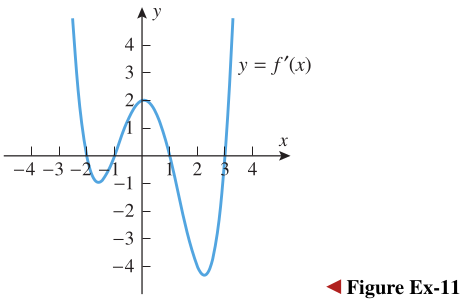
\includegraphics[width=0.6\textwidth]{../img/img_Lista2/3_11.png}
\end{figure}
La figura adjunta muestra la gráfica de $y = f'(x)$ para una función $f$ no especificada.
\begin{enumerate}[label=(\alph*)]
\item ¿Para qué valores de $x$ la curva $y = f(x)$ tiene una recta tangente horizontal?\\
  Dado que $y=f'(x)$ representa la pendiente de la recta tangente a $f(x)$, cuando $f'(x)=0$ la pendiente de la recta tangente es horizontal. Por tanto, los valores de $x$ son $-2,-1,1,3$.

\item ¿En qué intervalos la curva $y = f(x)$ tiene rectas tangentes con pendiente positiva?\\
  $(-\infty,-2),(-1,1),(3,+\infty)$.

\item ¿En qué intervalos la curva $y = f(x)$ tiene rectas tangentes con pendiente negativa?\\
  $(-2,-1), (1,3)$.

\item Dado que $g(x) = f(x) \sin x$, encuentre $g''(0)$.
  $$g'(x)=f(x)\cdot \cos x + \sin x \cdot f'(x)$$
  $$g''(x)=(-\sin xf(x) + cosxf'(x)) + (\sin xf''(x)+\cos xf'(x))$$
  \begin{equation*}
    \begin{split}
      g''(0)
      &= (-\sin 0 \cdot f(0) + cos0\cdot f'(0)) + (\sin 0\cdot f''(0)+\cos 0\cdot f'(0))\\
      &= f'(0) + f'(0) \\
      &= 2+2\\
      &=4
    \end{split}
  \end{equation*}
  
\end{enumerate}

%% 2 ---------------------------------------------------------------------------------------------------------------------------------------------------------------------------------------------------------------------------------
\section{Ejercicio 28} name \\

En cada parte, evalúa la expresión dado que $f(1)=1$, $g(1)=-2$, $f'(1)=3$ y $g'(1)=-1$.
\begin{enumerate}[label=(\alph*)]
\item $\frac{d}{dx} \lbrack f(x)g(x) \rbrack \vline _{x=1}$
  \begin{equation*}
    \begin{split}
      \frac{d}{dx} \left[ f(x)g(x) \right] \vline _{x=1}
      & = [f(x)g'(x)+g(x)f'(x)] \vline _{x=1} \\
      & = f(1)g'(1)+g(1)f'(1) \\
      & = (1 \cdot -1) + (-2 \cdot 3) \\
      & = -1 + (-6) \\
      & = -1-6 \\
      & =-7
    \end{split}
  \end{equation*}

\item $\frac{d}{dx} \lbrack \frac{f(x)}{g(x)} \rbrack \vline _{x=1}$
  \begin{equation*}
    \begin{split}
      \frac{d}{dx} \left [ \frac{f(x)}{g(x)} \right ] \vline _{x=1}
      & = \left[\frac{g(x)f'(x)-f(x)g'(x)}{\lbrack g(x) \right] ^2}] \vline _{x=1} \\
      & = \frac{g(1)f'(1)-f(1)g'(1)}{\lbrack g(1) \rbrack ^2}\\
      & = \frac{(-2 \cdot 3)-(1 \cdot -1)}{(-2) ^2}\\
      & = \frac{(-6)-(-1)}{4}\\
      & = \frac{-6+1}{4}\\
      & = - \frac{5}{4}\\
    \end{split}
  \end{equation*}

\item $\frac{d}{dx} \lbrack \sqrt{f(x)} \rbrack \vline _{x=1}$
  \begin{equation*}
    \begin{split}
      \frac{d}{dx} \left[ \sqrt{f(x)} \right] \vline _{x=1}
      & = \frac{d}{dx} { [f(x)]^{\frac{1}{2}} } \vline _{x=1} \\
      & = \left[ \frac{1}{2}[f(x)]^{-\frac{1}{2}} \cdot f'(x)\right] \vline _{x=1} \\
      & = \frac{1}{2}[f(1)]^{-\frac{1}{2}} \cdot f'(1)  \\
      & = \frac{1}{2}(1)^{-\frac{1}{2}} \cdot 3  \\
      & = \frac{1}{2}(1) \cdot 3  \\
      & = \frac{3}{2}
    \end{split}
  \end{equation*}

\item $\frac{d}{dx} \lbrack f(1)g'(1) \rbrack$
  \begin{equation*}
    \begin{split}
      \frac{d}{dx} \lbrack f(1)g'(1) \rbrack
      & = \frac{d}{dx} \lbrack 1 \cdot -1 \rbrack \\
      & = \frac{d}{dx} \lbrack -1 \rbrack \\
      & = 0
    \end{split}
  \end{equation*}
  
\end{enumerate}

%% 3 ---------------------------------------------------------------------------------------------------------------------------------------------------------------------------------------------------------------------------------
\section{Ejercicio 31} name \\

Encuentre $f'(x)$.
\begin{enumerate}[label=(\alph*)]
\item $f(x)=\sqrt{3x+1} (x-1)^2$
  \begin{equation*}
    \begin{split}
      f(x)
      &=\sqrt{3x+1} (x-1)^2\\
      &= (3x+1)^{\frac{1}{2}}(x-1)^2\\
      &= \left[ (3x+1)^{\frac{1}{2}} \cdot \frac{d}{dx}(x-1)^2 \right]
         + \left[ (x-1)^2 \cdot \frac{d}{dx}(3x+1)^{\frac{1}{2}} \right]\\
      &= \left\lbrace (3x+1)^{\frac{1}{2}} \left[ 2(x-1)\cdot \frac{d}{dx}(x-1)\right] \right\rbrace
         + \left\lbrace (x-1)^2\left[\frac{1}{2}(3x+1)^{-\frac{1}{2}}\cdot \frac{d}{dx}(3x+1)\right] \right\rbrace\\
      &= \left\lbrace (3x+1)^{\frac{1}{2}} \left[ 2(x-1)\cdot 1\right] \right\rbrace
         + \left\lbrace (x-1)^2\left[\frac{1}{2}(3x+1)^{-\frac{1}{2}}\cdot 3\right] \right\rbrace\\
         &= 2(x-1)(3x+1)^{\frac{1}{2}} + \frac{3(x-1)^2}{2(3x+1)^{\frac{1}{2}}}\\
         &= \frac{\left\lbrace2(3x+1)^{\frac{1}{2}}\left[2(x-1)(3x+1)^{\frac{1}{2}}\right]\right\rbrace
           + 3(x-1)^2}{2(3x+1)^{\frac{1}{2}}}\\
         &= \frac{4(x-1)(3x+1) + 3(x-1)^2}{2(3x+1)^{\frac{1}{2}}}\\
         &= \frac{(x-1)\left[ 4(3x+1)+3(x-1)  \right]}{2(3x+1)^{\frac{1}{2}}}\\
         &= \frac{(x-1)\left[ 12x+4+3x-3  \right]}{2(3x+1)^{\frac{1}{2}}}\\
         &= \frac{(x-1)(15x+1)}{2(3x+1)^{\frac{1}{2}}}\\
         &= \frac{(x-1)(15x+1)}{2\sqrt{3x+1}}\\
    \end{split}
  \end{equation*}
  
\item $f(x)=\left( \frac{3x+1}{x^2} \right)^3$
  \begin{equation*}
    \begin{split}
      f(x)
      &=\left( \frac{3x+1}{x^2} \right)^3\\
      &= 3\left( \frac{3x+1}{x^2} \right)^2 \frac{d}{dx}\left( \frac{3x+1}{x^2} \right)\\
      &= 3\left( \frac{3x+1}{x^2} \right)^2 \frac{d}{dx}\left[(3x+1)(x^{-2})\right]\\
      &= 3\left( \frac{3x+1}{x^2} \right)^2 \left[
      (3x+1)\frac{d}{dx}(x^{-2})+(x^{-2})\frac{d}{dx}(3x+1) \right]\\
      &= 3\left( \frac{3x+1}{x^2} \right)^2 \left[
      (3x+1)\frac{d}{dx}(x^{-2})+(x^{-2})\frac{d}{dx}(3x+1) \right]\\
      &= 3\left( \frac{3x+1}{x^2} \right)^2 \left[ (3x+1)(-2x^{-3})+(x^{-2})(3) \right]\\
      &= 3\cdot \frac{(3x+1)^2}{(x^2)^2} \left( -6x^{-2}-2x^{-3}+3x^{-2} \right)\\
      &= 3 \cdot \frac{(3x+1)^2}{x^4} \left( -3x^{-2}-2x^{-3} \right)\\
      &= -\frac{3(3x+1)^2}{x^4} \left( \frac{3}{x^2}+\frac{2}{x^3} \right)\\
      &= -\frac{3(3x+1)^2}{x^4} \left( \frac{3x+2}{x^3} \right)\\
      &= -\frac{3(3x+1)^2(3x+2)}{x^7} \\
    \end{split}
  \end{equation*}
  
\end{enumerate}

%% 4 ---------------------------------------------------------------------------------------------------------------------------------------------------------------------------------------------------------------------------------
\section{Ejercicio 41} name \\

Supongamos que $f'(x) = 2x \cdot f(x)$ y $f(2) = 5$.
\begin{enumerate}[label=(\alph*)]
\item Encuentra $g'(\pi / 3)$ si $g(x)=f(\sec x)$.
  \begin{equation*}
    \begin{split}
      g'(x)
      &= f'(\sec x)\frac{d}{dx}\sec x\\
      &= 2\sec x\cdot f(\sec x)\frac{d}{dx}\sec x\\
      &= 2\sec x\cdot f(\sec x)\cdot \sec x\tan x\\
      g'(\frac{\pi}{3})
      &= 2\sec \frac{\pi}{3}\cdot f(\sec \frac{\pi}{3})\cdot \sec \frac{\pi}{3}\tan \frac{\pi}{3}\\
      &= 2\cdot 2 \cdot f(2)\cdot 2\cdot \sqrt{3}\\
      &= 8\cdot 5 \sqrt{3}\\
      &= 40\sqrt{3}\\
    \end{split}
  \end{equation*}
  
\item Encuentra $h'(2)$ si $h(x)=\left[ f(x)/(x-1) \right]^4$.
  \begin{equation*}
    \begin{split}
      h'(x)
      &= 4\left(\frac{f(x)}{x-1}\right)^3\frac{(x-1)f'(x)-f(x)}{(x-1)^2}\\
      &= 4\left(\frac{f(x)}{x-1}\right)^3\frac{(x-1)(2x\cdot f(x))-f(x)}{(x-1)^2}\\
      &= 4\cdot \frac{[f(x)]^3}{(x-1)^3}\cdot \frac{f(x)[(x-1)(2x)-1]}{(x-1)^2}\\
      &= \frac{4[f(x)]^3}{(x-1)^3}\cdot \frac{f(x)(2x^2-2x-1)}{(x-1)^2}\\
      &= \frac{4[f(x)]^4(2x^2-2x-1)}{(x-1)^5}\\
      h'(2)
      &= \frac{4[f(2)]^4(2(2^2)-2\cdot 2-1)}{(2-1)^5}\\
      &= \frac{4(5)^4(2(4)-4-1)}{1^5}\\
      &= 4\cdot 625\cdot 3\\
      &= 7500
    \end{split}
  \end{equation*}
\end{enumerate}

%% 5 ---------------------------------------------------------------------------------------------------------------------------------------------------------------------------------------------------------------------------------
\section{Ejercicio 25} name \\

Utilice la diferenciación implícita para encontrar la pendiente de la recta tangente a la curva en el punto especificado y verifique que su respuesta sea consistente con la gráfica adjunta en la página siguiente.
\begin{equation*}
x^4+y^4=16; \qquad (1, \sqrt[4]15) \qquad \text{\textbf{[Lamé’s special quartic]}}
\end{equation*}
\begin{figure}[H]
\centering
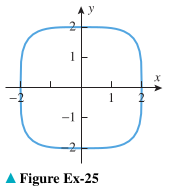
\includegraphics[width=0.35\textwidth]{../img/img_Lista2/3_25.png}
\end{figure}
Derivamos y con respecto de x
\begin{align*}
  4x^3+4y^3\frac{dy}{dx}=0\\
  4(x^3+y^3\frac{dy}{dx})=0\\
  x^3+y^3\frac{dy}{dx}=0\\
  \therefore \frac{dy}{dx}=-\frac{x^3}{y^3}
\end{align*}
Evaluamos en el punto $(1, \sqrt[4]15)$
\begin{equation*}
  \begin{split}
    \frac{dy}{dx}
    &=-\frac{x^3}{y^3} ~ \vline_{(1, \sqrt[4]15)}\\
    &= -\frac{1^3}{(\sqrt[4]15)^3}\\
    &= -\frac{1}{\sqrt[4]{15^3}}\\
    &\approx -0.1312\\
  \end{split}
\end{equation*}

%% 6 ---------------------------------------------------------------------------------------------------------------------------------------------------------------------------------------------------------------------------------
\section{Ejercicio 31} name \\

Utilice la diferenciación implícita para encontrar la derivada especificada.
\[ a^2 \omega^2 + b^2 \lambda^2 = 1 \text{ ($a$, $b$ constantes);}\qquad d\omega /d\lambda \]

Diferenciando implícitamente ambos lados de la ecuación con respecto a $\lambda$ produce
\begin{align*}
  2a^2\omega \frac{d\omega}{d\lambda}+2b^2\lambda=0\\
  2(a^2\omega \frac{d\omega}{d\lambda}+b^2\lambda)=0\\
  a^2\omega \frac{d\omega}{d\lambda}+b^2\lambda=0\\
  a^2\omega \frac{d\omega}{d\lambda}=-b^2\lambda\\
  \therefore \frac{d\omega}{d\lambda}=-\frac{b^2\lambda}{a^2\omega}\\
\end{align*}

%% 7 ---------------------------------------------------------------------------------------------------------------------------------------------------------------------------------------------------------------------------------
\section{Ejercicio 40} name \\

Se dice que dos curvas son \textbf{ortogonales} si sus rectas tangentes son perpendiculares en cada punto de intersección, y se dice que dos familias de curvas son \textbf{trayectorias ortogonales} entre sí si cada miembro de una familia es ortogonal a cada miembro de la otra familia. Esta terminología se utiliza en estos ejercicios.

La figura adjunta muestra algunos miembros típicos de las familias de hipérbolas $xy=c$ (curvas negras) y $x^2-y^2=k$ (curvas grises), donde $c \neq 0$ y $k \neq 0$. Utilice la sugerencia del ejercicio 39 para demostrar que estas familias son trayectorias ortogonales entre sí. [\textit{Sugerencia}: para que las rectas tangentes sean perpendiculares en un punto de intersección, las pendientes de esas rectas tangentes deben ser recíprocas negativas entre sí.]

\begin{figure}[H]
\centering
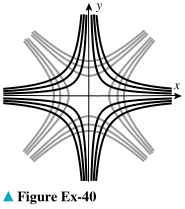
\includegraphics[width=0.35\textwidth]{../img/img_Lista2/3_40.png}
\end{figure}

Diferenciar implícitamente ambos lados de las siguientes ecuaciones con respecto a $x$ produce
\begin{enumerate}
\item $xy=c$
  \[ x\frac{dy}{dx}+1\cdot y=0 \]
  De la que obtenemos
  \begin{equation} \label{eqn: d_c_negras}
    \frac{dy}{dx}=-\frac{y}{x}
  \end{equation}

\item $x^2-y^2=k$
  \begin{align*} 
    2x - 2y\frac{dy}{dx}=0\\
    2(x-y\frac{dy}{dx})=0\\
    x-y\frac{dy}{dx}=0\\
  \end{align*}
  De la que obtenemos
  \begin{equation} \label{eqn: d_c_grises}
    \frac{dy}{dx}=\frac{x}{y}
  \end{equation}
\end{enumerate}

Al multiplicar las pendientes de las rectas tangentes de las familias de las hipérbolas, obtenemos\\
\[
  m_1 \cdot m_2 = -\frac{y}{x}\cdot \frac{x}{y}=-1\\
  \]
  
Por tanto, las pendientes de las rectas tangentes son recíprocas negativas entre sí, es decir:
  \[\therefore xy=c \perp x^2-y^2=k\]

Lo demostrado anteriormente aplica para cualquier valor dado de $x$ y $y$. No obstante, desarrollaremos los polinomios de las ecuaciones para encontrar los puntos de intersección de las curvas.\\

Sea $xy=c$, obtenemos que
\begin{equation} \label{eqn: y_c_negras}
y=\frac{c}{x}
\end{equation}

Sustituyendo el valor de $y$ de la ecuación \eqref{eqn: y_c_negras}

\begin{align*} 
  x^2-y^2=k \underset{y=\frac{c}{x}}{\Longrightarrow} x^2- \left( \frac{c}{x} \right) ^2=k\\
  x^2-\frac{c^2}{x^2}-k=0\\
  x^4-kx^2-c^2=0
\end{align*}

Por lo tanto, los valores de $x$ son

\begin{align*}
  x_0=\sqrt{\frac{k+\sqrt{k^2+4c^2}}{2}}\\
  x_1=-\sqrt{\frac{k+\sqrt{k^2+4c^2}}{2}}\\
  x_2=\sqrt{\frac{k-\sqrt{k^2+4c^2}}{2}}\\
  x_3=-\sqrt{\frac{k-\sqrt{k^2+4c^2}}{2}}\\
\end{align*}

Sustituyendo el valor de cada $x$ en la ecuación \eqref{eqn: y_c_negras}, obtenemos los valores de y para cada valor de $x$
\begin{align*}
  y_0=\frac{1}{c}\sqrt{\frac{k+\sqrt{k^2+4c^2}}{2}}\\
  y_1=-\frac{1}{c}\sqrt{\frac{k+\sqrt{k^2+4c^2}}{2}}\\
  y_2=\frac{1}{c}\sqrt{\frac{k-\sqrt{k^2+4c^2}}{2}}\\
  y_3=-\frac{1}{c}\sqrt{\frac{k-\sqrt{k^2+4c^2}}{2}}\\
\end{align*}

Ahora, evaluamos cada punto de intersección en la derivada de la ecuación $xy=c$
\begin{equation*}
  \begin{split}
    \frac{dy}{dx}
    &= -\frac{y}{x} ~ \vline _{(x_0,y_o)}\\
    &=  -\frac{y}{x} ~ \vline _{\left(\sqrt{\frac{k+\sqrt{k^2+4c^2}}{2}}, \frac{1}{c}\sqrt{\frac{k+\sqrt{k^2+4c^2}}{2}}\right)}\\
    &= -\frac{\frac{1}{c}\sqrt{\frac{k+\sqrt{k^2+4c^2}}{2}}}{\sqrt{\frac{k+\sqrt{k^2+4c^2}}{2}}}\\
    &= -\frac{1}{c}\\
  \end{split}
\end{equation*}
\begin{equation*}
  \begin{split}
    \frac{dy}{dx}
    &= -\frac{y}{x} ~ \vline _{(x_1,y_1)}\\
    &=  -\frac{y}{x} ~ \vline _{\left(-\sqrt{\frac{k+\sqrt{k^2+4c^2}}{2}}, -\frac{1}{c}\sqrt{\frac{k+\sqrt{k^2+4c^2}}{2}}\right)}\\
    &= -\frac{\frac{1}{c}\left(-\sqrt{\frac{k+\sqrt{k^2+4c^2}}{2}}\right)}{-\sqrt{\frac{k+\sqrt{k^2+4c^2}}{2}}}\\
    &= -\frac{1}{c}\\
  \end{split}
\end{equation*}
\begin{equation*}
  \begin{split}
    \frac{dy}{dx}
    &= -\frac{y}{x} ~ \vline _{(x_2,y_2)}\\
    &=  -\frac{y}{x} ~ \vline _{\left(\sqrt{\frac{k-\sqrt{k^2+4c^2}}{2}}, \frac{1}{c}\sqrt{\frac{k-\sqrt{k^2+4c^2}}{2}}\right)}\\
    &= -\frac{\frac{1}{c}\sqrt{\frac{k-\sqrt{k^2+4c^2}}{2}}}{\sqrt{\frac{k-\sqrt{k^2+4c^2}}{2}}}\\
    &= -\frac{1}{c}\\
  \end{split}
\end{equation*}
\begin{equation*}
  \begin{split}
    \frac{dy}{dx}
    &= -\frac{y}{x} ~ \vline _{(x_3,y_3)}\\
    &=  -\frac{y}{x} ~ \vline _{\left(-\sqrt{\frac{k-\sqrt{k^2+4c^2}}{2}}, -\frac{1}{c}\sqrt{\frac{k-\sqrt{k^2+4c^2}}{2}}\right)}\\
    &= -\frac{\frac{1}{c}\left(-\sqrt{\frac{k-\sqrt{k^2+4c^2}}{2}}\right)}{-\sqrt{\frac{k-\sqrt{k^2+4c^2}}{2}}}\\
    &= -\frac{1}{c}\\
  \end{split}
\end{equation*}

Enseguida, evaluamos cada punto de intersección en la derivada de la ecuación $x^2-y^2=k$
\begin{equation*}
  \begin{split}
    \frac{dy}{dx}
    &= \frac{x}{y} ~ \vline _{(x_0,y_o)}\\
    &= \frac{x}{y} ~ \vline _{\left(\sqrt{\frac{k+\sqrt{k^2+4c^2}}{2}}, \frac{1}{c}\sqrt{\frac{k+\sqrt{k^2+4c^2}}{2}}\right)}\\
    &= \frac{\sqrt{\frac{k+\sqrt{k^2+4c^2}}{2}}}{\frac{1}{c}\sqrt{\frac{k+\sqrt{k^2+4c^2}}{2}}}\\
    &= c\\
  \end{split}
\end{equation*}
\begin{equation*}
  \begin{split}
    \frac{dy}{dx}
    &= \frac{x}{y} ~ \vline _{(x_1,y_1)}\\
    &= \frac{x}{y} ~ \vline _{\left(-\sqrt{\frac{k+\sqrt{k^2+4c^2}}{2}}, -\frac{1}{c}\sqrt{\frac{k+\sqrt{k^2+4c^2}}{2}}\right)}\\
    &= \frac{-\sqrt{\frac{k+\sqrt{k^2+4c^2}}{2}}}{\frac{1}{c}\left(-\sqrt{\frac{k+\sqrt{k^2+4c^2}}{2}}\right)}\\
    &= c\\
  \end{split}
\end{equation*}

\end{document}
